% ------------------------------------------------------------------
\renewcommand{\thisunit}{MATH327 Unit 1}
\renewcommand{\moddate}{Last modified 5 Feb.~2023}
\setcounter{section}{1}
\setcounter{subsection}{0}
\phantomsection
\addcontentsline{toc}{section}{Unit 1: Central limit theorem and diffusion}
\section*{Unit 1: Central limit theorem and diffusion}
\subsection*{Introductory remarks: What is Statistical Physics?}
Mathematical sciences such as physics aim to determine the laws of nature and understand how these govern experimental observations --- both in everyday circumstances and under extreme conditions.
This mathematical understanding is typically guided by reproducing a set of observations, with the resulting framework then used to make predictions for other ``observables''.

Over the past few centuries this process has been tremendously successful, with theoretical physics accurately predicting experimental and observational results from sub-atomic through to supra-galactic scales.
Modern physics labs can create a vacuum better than in outer space and the coldest temperatures in the known universe, as well as going to the other extreme to reach temperatures of millions of degrees and pressures millions of times atmospheric pressure at sea level.
Amazingly, many aspects of these realms of physics can be theoretically described by mathematics developed centuries ago.\footnote{Eugene Wigner's famous article, ``\href{https://en.wikipedia.org/wiki/The_Unreasonable_Effectiveness_of_Mathematics_in_the_Natural_Sciences}{The Unreasonable Effectiveness of Mathematics in the Natural Sciences}'' (1960), and subsequent work in the philosophy of physics, elaborates on why this may be considered `amazing'.  This module will not comment extensively on philosophy.}

Statistical physics is one domain in which simple mathematical principles enable amazing predictive capabilities.
Initially developed in the nineteenth century, statistical physics remains a central pillar of modern physics, and will retain this position in years to come.
The foundations of statistical physics lie in the use of probability theory to mathematically describe experimental observations and corresponding laws of nature that involve stochastic randomness rather than being perfectly predictable.

The lack of perfect predictability in statistical physics is a matter of practicality rather than one of principle.
It results from working with a large number of degrees of freedom --- that is, a large number of independent objects such as atoms.
For illustration, Avogadro's number $N_A \approx 6.022\times 10^{23}$ is the large number of molecules in everyday amounts of familiar substances --- about 18~grams of water or about 22~litres of air at sea-level atmospheric pressure ($\approx$$101$~kPa). % 22.4 litres for 1atm=101.325~kPa, 22.71 litres for 100~kPa at $O^{\circ}$~C
Specifying the positions and velocities of $\sim$$10^{23}$ objects would require far more information than could be stored even in the memory of the biggest existing supercomputers.
Statistical physics instead produces simple mathematical descriptions of large-scale properties such as temperature, pressure and diffusion, which are generally of such outstanding quality that the underlying `randomness' is effectively invisible.

Historically, the difficulty of detecting the stochastic processes underlying such \textit{thermodynamic} properties made it challenging to convince skeptics that atoms and molecules really exist.
\href{https://en.wikipedia.org/wiki/Ludwig_Boltzmann}{Ludwig Boltzmann}, a prominent early developer of statistical physics, endured a constant struggle to defend his ideas, which likely contributed to his deteriorating mental health and eventual suicide in 1906.
A significant step to convincingly establish the existence of atoms was Albert Einstein's use of statistical physics to explain the observed ``\href{https://en.wikipedia.org/wiki/Brownian_motion}{Brownian motion}'' of particles suspended in fluids --- this work was part of Einstein's ``miracle year'' in 1905, along with special relativity and early contributions to quantum physics.
\href{https://en.wikipedia.org/wiki/Jean_Baptiste_Perrin}{Jean Perrin} soon verified Einstein's predictions and used them to determine Avogadro's number; he was awarded the 1926 Nobel Prize in Physics for helping to demonstrate ``the discontinuous structure of matter''.
More recently, applications of statistical physics to advance our ``understanding of complex physical systems'' were recognized by the \href{https://www.nobelprize.org/prizes/physics/2021/summary/}{2021 Nobel Prize in Physics} shared between Syukuro Manabe, Klaus Hasselmann and Giorgio Parisi.
Other modern topics we will encounter in this module include explaining why stars don't collapse under the `weight' of their own gravity, and identifying effects of dark matter in temperature fluctuations observable in the \textit{cosmic microwave background} lingering from the early years of the universe.

In this unit we will focus on some of the foundational mathematics that will underlie our later development and application of statistical ensembles.
Looking back to Boltzmann's times, we can consider the following question one of his critics might have asked:
\textit{If the pressure of a gas in a container results from molecules stochastically colliding with the walls of that container, then how can the pressure be so stable and reproducible, rather than itself fluctuating stochastically?}
The mathematical answer lies in the \textbf{law of large numbers} and the \textbf{central limit theorem}, which we will review and apply to the physics of diffusion in one dimension.
% ------------------------------------------------------------------



% ------------------------------------------------------------------
\subsection{\label{sec:prob}Probability foundations}
We begin by building a more formal mathematical framework around the concept of probability, through a sequence of definitions.

First, a random \textbf{experiment} \cE involves setting up, manipulating and/or observing some (physical or hypothetical) system with some element of randomness.
Flipping a coin is a simple random experiment.
In the context of the statistical ensembles that will be the focus of this module, a typical experiment will be to allow a collection of particles to evolve in time, subject to certain constraints.

Each time an experiment is performed, the world comes out in some \textbf{state} $\om$.
The specification of the experiment and the state must include all objects of interest, and may include more besides.
When flipping a coin, for example, the full state could contain information not only about the final orientation of the coin, but also about its position --- did it land on the ground or was it caught?

The \textbf{set of all states} \Om collects all possible states \om that the given experiment \cE can produce, and is therefore intricately tied to \cE itself.

We are generally not interested in all aspects of the full state $\om$.
For example, we won't care where a flipped coin lands.
Instead we're typically only interested in whether it lands heads up or tails up --- and we may want to set aside any state that doesn't cleanly reflect those options.
The \textbf{measurement} $X(\om)$ extracts and quantifies this information, acting as a function that maps the state \om to a number that we can mathematically manipulate.
If we repeat the given experiment \cE many times and carry out the measurement $X$ on each resulting state $\om_i$, we will obtain a sequence of numbers $X(\om_i)$ that behave as a \textit{random variable}.

Acting with the measurement $X$ on all of the possible states in the set \Om defines the \textbf{set of all outcomes} (or \textbf{outcome space}) $A$:
\begin{equation*}
  X: \Om \to A.
\end{equation*}
That is, $A$ collects all possible measurement results that the given experiment \cE and measurement $X$ can produce.
$A$ can be finite, countably infinite, or uncountably infinite (i.e., continuous).

Let's consider some examples to clarify these definitions.
With an experiment of rolling a six-sided die and measuring the number ($1$--$6$) that comes out on top, what is the set of all outcomes $A$?
What additional information could be included in a corresponding state $\om$?
\begin{mdframed}
  \ \\[75 pt] % WARNING: ADJUSTED SIZE BY HAND TO FIT ON PAGE
\end{mdframed}
What is the outcome space $A$ if we toss a coin four times and measure whether it lands heads up ($H$) or tails up ($T$) each time? % Note four tosses is being defined as a single experiment...
\begin{mdframed}
  \ \\[75 pt] % WARNING: ADJUSTED SIZE BY HAND TO FIT ON PAGE
\end{mdframed}
What information could characterize a state \om for a gas of $10^{23}$ argon atoms in a container?
What might be interesting to measure?
\begin{mdframed}
  \ \\[95 pt] % WARNING: ADJUSTED SIZE BY HAND TO FIT ON PAGE
\end{mdframed}

We can generalize the concept of measurement by introducing a unique number as a \textit{label} to characterize each state \om in the set $\Om$.
This would provide a label function $L(\om)$ as a random variable.
Our condition of uniqueness makes $L(\om)$ isomorphic, so that the label can be used interchangeably with the full state,
\begin{equation*}
  \om \llra L(\om).
\end{equation*}
While the measurements $X(\om)$ we consider generally will not produce a unique number for each $\om$, we will design them precisely to remove irrelevant information that doesn't interest us.
Ignoring that irrelevant information leaves us free to interchange the set of outcomes $A$ for the set of states $\Om$.
(Some textbooks may never distinguish between $A$ vs \Om in the first place, though this can be a source of confusion.)

Only a couple of definitions remain.
The next is to define an \textbf{event} to be any subset of the set of all outcomes $A$.
For example, events resulting from rolling a die could include (i) rolling a $6$, (ii) rolling anything but a $6$, (iii) rolling any even number, and many more.
Collecting all events of interest defines the \textbf{set of events} (or \textbf{event space}) $\cF$.

We are now prepared for the final foundational definition in this section, the \textbf{probability} $P$ of an event in the set $\cF$.
Mathematically, $P$ is a \textit{measure function},
\begin{equation*}
  P: \cF \to [0, 1],
\end{equation*}
which must satisfy the following two requirements: \\[-24 pt]
\begin{enumerate}
  \item The probability of a countable union of mutually exclusive events must equal the sum of the probabilities of each of these events.
  \item The probability of the outcome space ($\cF = A$) must equal $1$, even if $A$ is uncountable.
        This simply means that the experiment \cE must produce a measurable outcome.
        We discard any experiment that doesn't produce such an outcome. \\[-24 pt]
\end{enumerate}
Combining the outcome space, event space and probability measure gives us a \textit{probability space} $(A, \cF, P)$.

For example, consider an experiment that can only produce $N$ possible states, so that
\begin{equation*}
  \Om = \left\{\om_1, \om_2, \cdots, \om_N\right\}.
\end{equation*}
As described above, it is possible for two different states $\om_i \ne \om_j$ to produce the same measurement outcome $X(\om_i) = X(\om_j)$.
This means that the size $n$ of the outcome space $A$ may be smaller than the size of $\Om$, $n \leq N$.
We can write
\begin{equation*}
  A = \left\{X_1, X_2, \cdots, X_n\right\},
\end{equation*}
where each $X_{\al}$ is distinct and its index does not necessarily correspond to that on $\om_i$.
We can take the individual $X_{\al}$ themselves to be the events we're interested in, choosing the event space
\begin{equation}
  \label{eq:finite_set}
  \cF = \left\{X_1, X_2, \cdots, X_n\right\} = A.
\end{equation}
These events are all mutually exclusive by construction, so if we assign them probabilities
\begin{equation*}
  P(X_{\al}) \equiv p_{\al} \qquad \mbox{for } \al = 1, \cdots, n,
\end{equation*}
then the above requirements on probabilities demand that for any $\al \ne \be$ we have
\begin{align*}
  P(X_{\al} \mbox{ or } X_{\be}) & = p_{\al} + p_{\be} \\
  P(A) = P(X_1 \hbox{ or } X_2 \hbox{ or } \cdots \mbox{ or } X_n) & = \sum_{\al = 1}^n p_{\al} = 1.
\end{align*}

Similarly choosing an event space $\cF = A$ for the six-sided die considered in an earlier gap, what are the probabilities $p_1$ through $p_6$ that result from assuming the die is fair?
\begin{mdframed}
  \ \\[100 pt]
\end{mdframed}
Again taking $\cF = A$ for the case of tossing a coin four times, what are the probabilities $p_{\al}$ that result from assuming the coin is fair?
If we instead consider the event space
\begin{equation*}
  \cF = \left\{\mbox{equal number of } H \mbox{ and } T, \mbox{ different numbers of } H \mbox{ and } T\right\},
\end{equation*}
what are the probabilities $p_{\text{equal}}$ and $p_{\text{diff}}$ for the two events in this $\cF$?
\begin{mdframed}
  \ \\[100 pt]
\end{mdframed}

\newpage % WARNING: FORMATTING BY HAND
\begin{minipage}{0.4\textwidth}
  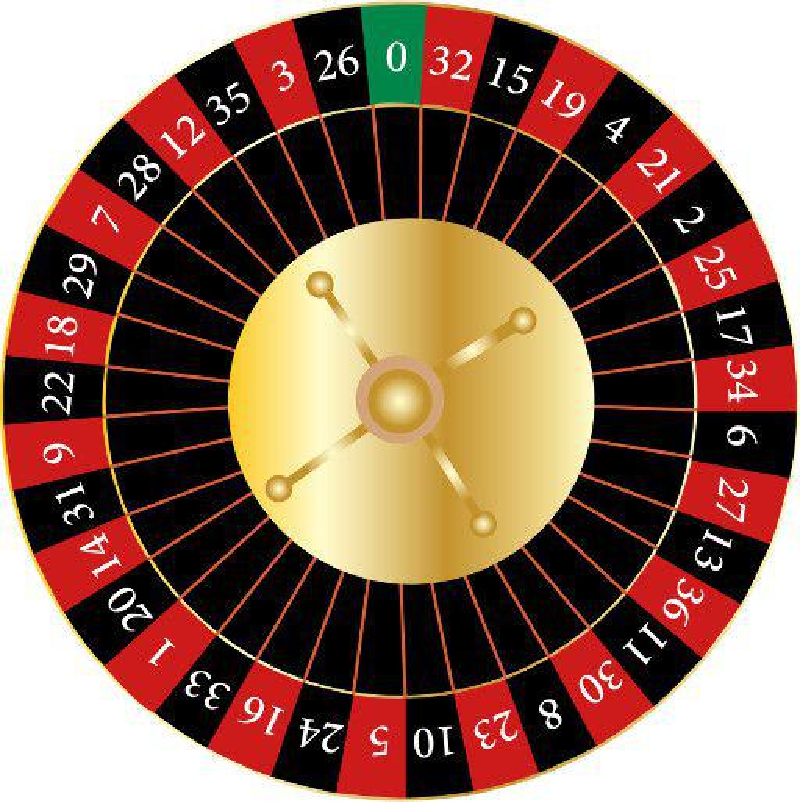
\includegraphics[width=0.75\textwidth]{figs/unit01_roulette.pdf}
\end{minipage}%
\begin{minipage}{0.5\textwidth}
  The standard European roulette wheel shown to the left (\href{https://www.vecteezy.com/vector-art/658761-casino-roulette-wheel}{source}) has 37 pockets labelled ``0'' through ``36''.
  18 of these pockets are coloured red, 18 are coloured black and 1 (pocket ``0'') is coloured green.
  Note that measuring the label automatically provides the colour.
\end{minipage}

\noindent What is the outcome space $A$ for a spin of the roulette wheel?
With $\cF = A$, what are the probabilities $p_{\al}$ for a fair wheel?
With
\begin{equation*}
  \cF = \left\{\mbox{ball in a red pocket, ball in a black pocket, ball in the green pocket}\right\},
\end{equation*}
what are the corresponding probabilities $p_{\text{red}}$, $p_{\text{black}}$ and $p_{\text{green}}$?
\begin{mdframed}
  \ \\[100 pt]
\end{mdframed}

The process of assigning probabilities to events is called \textit{modelling}.
In the gaps above we saw above that \textit{symmetries} are a powerful way to constrain probabilities.
The symmetry between the six sides of a fair die, the two sides of a fair coin, and the 37 pockets of a fair roulette wheel each sufficed to completely fix the corresponding probabilities $p_{\al}$.

Modelling can also be guided by empirical data obtained by repeating an experiment many times.
For example, if we don't know whether a set of dice are fair, we will be able to infer their probabilities $p_{\al}$ (with a certain confidence level) by rolling them enough times.
The need to repeat the experiment many times comes from the law of large numbers, to which we now turn.
% ------------------------------------------------------------------



% ------------------------------------------------------------------
\subsection{\label{sec:LLN}Law of large numbers}
Let's return to the setup leading to \eq{eq:finite_set} above, with
\begin{equation*}
  \cF = A = \left\{X_1, X_2, \cdots, X_n\right\}
\end{equation*}
for finite $n$, and probabilities $p_{\al} = P(X_{\al})$ that obey
\begin{align*}
  p_{\al} & \in [0, 1] &
  \sum_{\al = 1}^n p_{\al} & = 1.
\end{align*}
We can generalize this notation by writing instead
\begin{equation*}
  \sum_{X \in A} P(X) = 1,
\end{equation*}
which provides simple expressions for the \textbf{mean} $\mu$ and \textbf{variance} $\si^2$ of the probability space,
\begin{align}
              \mu = \vev{X} = & \sum_{X \in A} X \, P(X)            \label{eq:mean} \\
  \si^2 = \vev{(X - \mu)^2} = & \sum_{X \in A} (X - \mu)^2 \, P(X). \label{eq:var}
\end{align}
The angle bracket notation indicates the \textbf{expected} (or \textbf{expectation}) \textbf{value} with general definition
\begin{equation}
  \label{eq:expect_disc}
  \vev{f(X)} = \sum_{X \in A} f(X) \, P(X),
\end{equation}
which is a linear operation,
\begin{equation*}
  \vev{c\cdot f(X) + g(X)} = c\vev{f(X)} + \vev{g(X)}.
\end{equation*}
The square root of the variance, $\sqrt{\si^2} = \si$, is the \textbf{standard deviation}.
What is \si expressed in terms of $\vev{X^2}$ and $\vev{X}^2$?
\begin{mdframed}
  \ \\[100 pt]
\end{mdframed}

We now define a new experiment that consists of \textit{repeating} the original experiment $R$ times, with each repetition independent of all the others.
Using the same measurement as before for each repetition, we obtain a new outcome space that we can call $B$.
For $R = 4$, what are some representative outcomes in the set $B$?
What is the total size of $B$?
\begin{mdframed}
  \ \\[100 pt]
\end{mdframed}

Each outcome in $B$ contains $R$ different $X^{(r)} \in A$, one for each repetition $r = 1, \cdots, R$, and each with mean $\vev{X^{(r)}} = \mu$ and variance $\vev{(X^{(r)} - \mu)^2} = \si^2$.
Considering the case $R = 4$ for simplicity, any element of $B$ can be written as $X_i^{(1)} X_j^{(2)} X_k^{(3)} X_l^{(4)} \in B$ with corresponding probability
\begin{equation*}
  P_B\left(X_i^{(1)} X_j^{(2)} X_k^{(3)} X_l^{(4)}\right) = P_A\left(X_i^{(1)}\right) P_A\left(X_j^{(2)}\right) P_A\left(X_k^{(3)}\right) P_A\left(X_l^{(4)}\right),
\end{equation*}
using subscripts to distinguish between the single-experiment ($A$) and repeated-experiment ($B$) probability spaces.

Averaging over all $R$ repetitions defines the \textit{arithmetic mean}
\begin{equation}
  \label{eq:ave}
  \Xbar_R = \frac{1}{R} \sum_{r = 1}^R X^{(r)}.
\end{equation}
Unlike the true mean $\mu$, the arithmetic mean $\Xbar_R$ is a random variable --- a number that may be different for each element of $B$.
That said, $\Xbar_R$ and $\mu$ are certainly related, and so long as the standard deviation exists --- that is, so long as $\si^2$ is finite --- this relation can be proved rigorously in the limit $R \to \infty$.\footnote{In the computer project we will numerically investigate a situation where $\si^2$ diverges.}

Here we will not be fully rigorous, and take it as given that
\begin{equation*}
  \vev{\left(X^{(i)} - \mu\right)\left(X^{(j)} - \mu\right)} = \si^2 \de_{ij} = \left\{\begin{array}{ll}\si^2 & \mbox{for } i = j \\ 0 & \mbox{for } i \ne j\end{array}\right.,
\end{equation*}
where the \textit{Kronecker delta} $\de_{ij} = 1$ for $i = j$ and vanishes for $i \ne j$.
This is a consequence of the assumed independence of the different repetitions.
Using this result and the relation $\big(\sum_i a_i\big)\big(\sum_j b_j\big) = \sum_{i, j} \left(a_i b_j\right)$, express the following quantity in terms of \si and $R$:
\begin{mdframed}
  $\displaystyle \vev{\left(\frac{1}{R} \sum_{r = 1}^R X^{(r)} - \mu\right)^2} = $ \\[100 pt] % TODO: More space here might be convenient...
\end{mdframed}
You should find that your result vanishes in the limit $R \to \infty$, so long as $\si^2$ is finite.
Since the square makes this expectation value a sum of non-negative terms, it can vanish only if every one of those terms is individually zero.

\begin{shaded}
  This establishes the \textbf{law of large numbers}:
  \begin{equation}
    \lim_{R \to \infty} \frac{1}{R} \sum_{r = 1}^R X^{(r)} = \mu,
  \end{equation}
  where we have assumed $\vev{X^{(r)}} = \mu$ and $\vev{(X^{(r)} - \mu)^2} = \si^2$ are finite.
\end{shaded}
% ------------------------------------------------------------------



% ------------------------------------------------------------------
\subsection{\label{sec:probdist}Probability distributions}
It is not necessary to make the assumption (\eq{eq:finite_set}) that our outcome space contains only a countable number of possible outcomes.
The considerations above continue to hold even if the random variable $X$ is a continuous real number.
In this case, however, the identification of probabilities with outcomes is slightly more complicated, which will be relevant when we consider the central limit theorem in the next section.

When the outcome can be any number on the real line, the fundamental object is a \textbf{probability distribution} (or \textbf{density function}) $p(x)$ defined for all $x \in \Rbb$.
Starting from this density, a probability is determined by integrating over a given interval.
Calling this interval $[a, b]$, the integration produces the probability that the outcome $X$ lies within the interval,
\begin{equation*}
  P\left(a \leq X \leq b\right) = \int_a^b p(x) \; dx.
\end{equation*}

We similarly generalize the definition of an expectation value (\eq{eq:expect_disc}) to an integral over the entire domain of the  probability distribution,
\begin{equation*}
  \vev{f(x)} = \int f(x) \; p(x) \; dx.
\end{equation*}
We will omit the limits on integrals over the entire domain, so for $x \in \Rbb$ we implicitly have $\int dx = \int_{-\infty}^{\infty} dx$, with $\int p(x) \; dx = 1$.
An important set of expectation values is
\begin{equation}
  \label{eq:expect_cont}
  \vev{x^{\ell}} = \int x^{\ell} \; p(x) \; dx,
\end{equation}
which provides the mean and variance of the probability distribution $p(x)$, through generalizations of Eqs.~\ref{eq:mean}--\ref{eq:var}:
\begin{align}
  \label{eq:mean_var}
  \mu   & = \vev{x} = \int x \; p(x) \; dx &
  \si^2 & = \vev{x^2} - \vev{x}^2.
\end{align}
The expression for the variance should be familiar from your determination of the standard deviation in an earlier gap.
Unless stated otherwise, we will assume the mean and variance are both finite for the probability distributions we consider.
% ------------------------------------------------------------------



% ------------------------------------------------------------------
\subsection{\label{sec:CLT}Central limit theorem}
The central limit theorem is a central result of probability theory (hence its name).
Over the years it has been expressed in several equivalent ways, and there are also many distinct variants of the theorem accommodating different conditions and assumptions.
In this module we are interested in applying rather than proving the central limit theorem; you can find \href{https://en.wikipedia.org/wiki/Central_limit_theorem#Proof_of_classical_CLT}{proofs} in many textbooks.

The version of the theorem we use in this module assumes we have $N$ independent random variables $x_1, \cdots, x_N$, each of which has the same (finite) mean $\mu$ and variance $\si^2$.
Such random variables are said to be \textit{identically distributed}, and a common way to obtain them is to repeat an experiment $N$ times, as we considered in \secref{sec:LLN}.
Just as in \eq{eq:ave}, the sum
\begin{equation}
  \label{eq:CLTsum}
  s = \sum_{i = 1}^N x_i
\end{equation}
is itself a random variable.

\begin{shaded}
  The \textbf{central limit theorem} states that for large $N \gg 1$ the probability distribution for $s$ is
  \begin{equation}
    \label{eq:CLT}
    p(s) \approx \frac{1}{\sqrt{2\pi N\si^2}} \exp\left[-\frac{(s - N\mu)^2}{2N\si^2}\right],
  \end{equation}
  with the approximation becoming exact in the $N \to \infty$ limit.
\end{shaded}
In addition to asserting that the collective behaviour of many independent and identically distributed random variables $x_i$ is governed by a \textbf{normal} (or \textbf{gaussian}) \textbf{distribution}, the central limit theorem further specifies the precise form of this distribution in terms of the mean and variance of \textit{each individual} $x_i$. % TODO: Could explicitly emphasize connection to big picture of statistical physics...

\begin{minipage}{0.55\textwidth}
  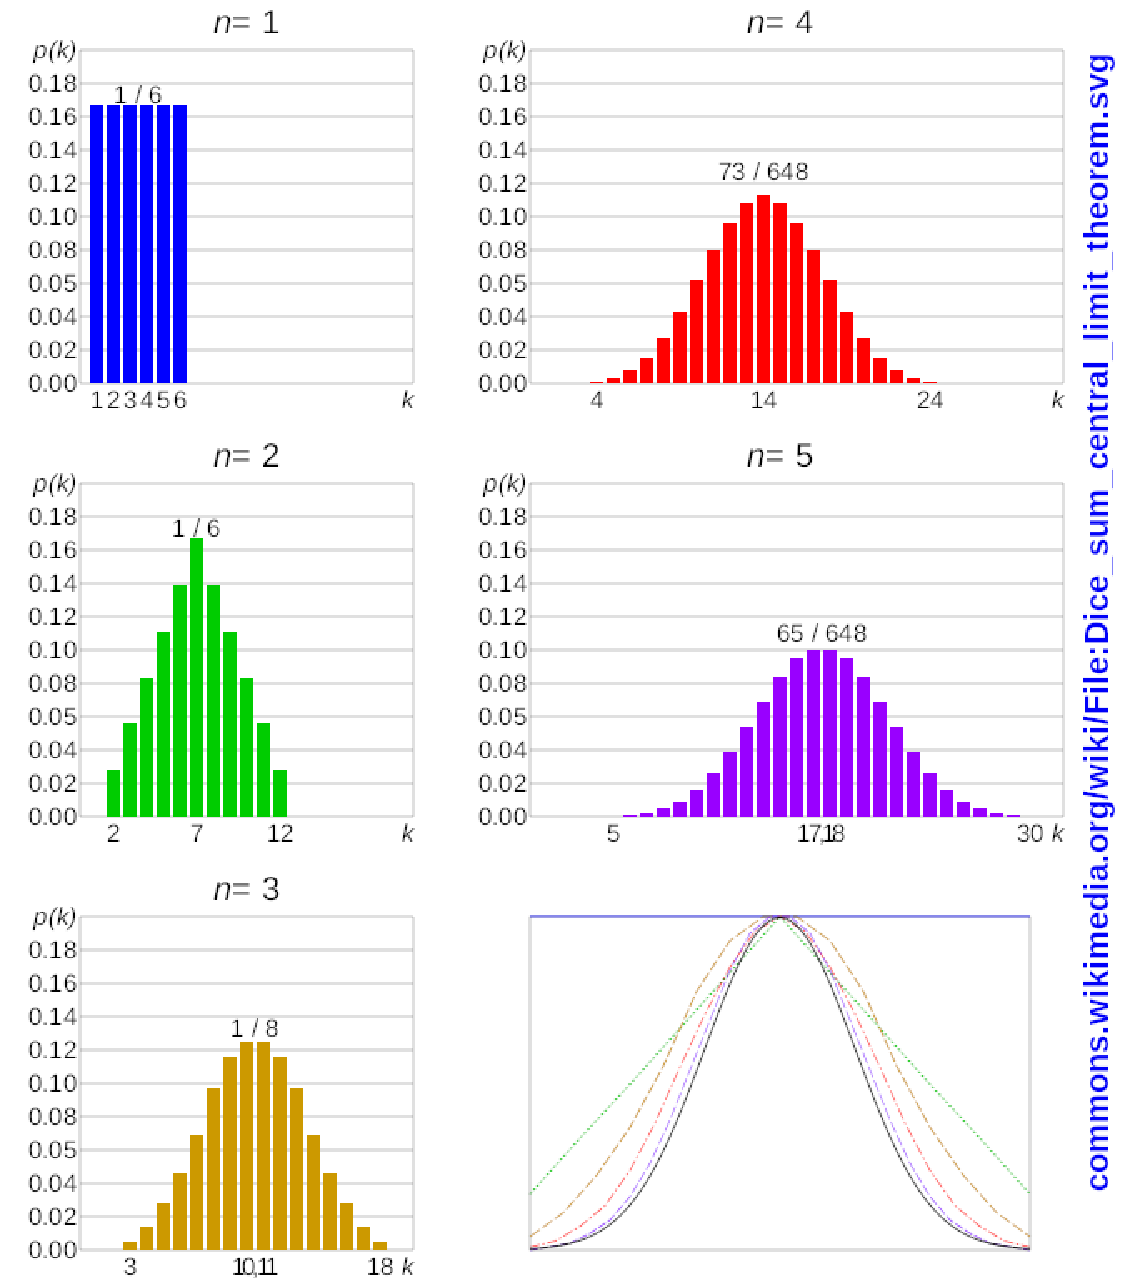
\includegraphics[width=0.8\textwidth]{figs/unit01_CLT.pdf}
\end{minipage}%
\begin{minipage}{0.35\textwidth}
  In practice, $N$ often doesn't need to be very large in order for the central limit theorem to provide a reasonable approximation.
  This is illustrated by the figure to the left, from \href{https://commons.wikimedia.org/wiki/File:Dice_sum_central_limit_theorem.svg}{{Wikimedia Commons}}, which shows the probabilities for the sum of $n \leq 5$ rolls of a six-sided die rapidly approaching a gaussian distribution.
\end{minipage}
% ------------------------------------------------------------------



% ------------------------------------------------------------------
\subsection{\label{sec:diffusion}Diffusion and the central limit theorem}
\subsubsection{Random walk on a line}
As a more powerful application and illustration of the central limit theorem, let's consider the behaviour of a randomly moving object.
Such \textbf{random walks} appear frequently in mathematical modelling of stochastic phenomena (including Brownian motion), and can be applied to movement through either physical space or more abstract vector spaces.
They are examples of \href{https://en.wikipedia.org/wiki/Markov_process}{Markov processes}, in which the state of the system (in this case the position of the `walker') at any time probabilistically depends only on the system's prior state at the previous point in time --- there is no `memory' of any earlier states. % Named after \href{https://en.wikipedia.org/wiki/Andrey_Markov}{Andrey Markov}...
The resulting sequence of system states is known as a \textit{Markov chain}, since each state is produced from the one before, like links in a chain.

Let's consider the simple example of a random walker that moves only in a single spatial dimension --- to the left or to the right on a line --- and can only take `steps' of a fixed length, which we can set to $\ell = 1$ without loss of generality.
At each point in time, the walker takes either a step to the right ($R$) with probability $p$ or a step to the left ($L$) with probability $q = 1 - p$.
We will further assume that each step takes a constant amount of time $\De t$, so a walk of $N$ steps will last for total time
\begin{equation}
  \label{eq:RWtime}
  t = N \De t.
\end{equation}

As an example, for $N = 6$ a representative walk can be written as $LRLRRR$, which leaves the walker $x = 2$ steps to the right of its starting point ($x = 0$).
The opposite walk $RLRLLL$ would leave the walker at $x = -2$, with negative numbers indicating positions to the left of the starting point.
How many possible walks are there for $N = 6$, and what is the probability (in terms of $p$ and $q$) for these particular walks $LRLRRR$ and $RLRLLL$ to occur?
How many possible walks are there for general $N$, and what is the probability for any particular walk involving $r$ steps to the right to occur?
\begin{mdframed}
  \ \\[100 pt]
\end{mdframed}

We will be interested in the walker's final position $x$ at time $t$ after it has taken $N$ steps.
Just as for the sum of $n$ rolls of a die considered in \secref{sec:CLT}, there are a range of possible final positions $x$, each of which has some probability $P(x)$ of being realized.
The key pieces of information we want to determine are the expectation value $\vev{x}$ and the variance $\vev{x^2} - \vev{x}^2$ that indicates the scale of fluctuations we can expect around $\vev{x}$ as the $N$-step walk is repeated many times from the same starting point.
(We reserve the variables $\mu$ and $\si^2$ for the respective mean and variance of the single-step process, which will appear when we apply the central limit theorem in \secref{sec:RW_CLT}.)

Suppose the $N$ total steps involve $r$ steps to the right.
What is the final position $x$ of the walker in terms of $N$ and $r$?
Check your general answer for the cases $N = 6$ and $r = 4$, $2$ considered above.
\begin{mdframed}
  \ \\[80 pt]
\end{mdframed}
This relation makes it equivalent to consider either the probability $P_r$ of taking $r$ steps to the right, or the probability $P(x)$ of ending up at final position $x$.
This equivalence will not hold for more general random walks in which the step length is no longer fixed and $\ell_i$ can vary from one step to the next.

Because the order in which steps are taken does not affect the final position $x$, to determine the probability $P(x)$ we have to count all possible ways of walking to $x$.
For $N = 6$, what are all the possible walks that produce $x = 4$, and what is the corresponding probability $P(4)$?
\begin{mdframed}
  \ \\[100 pt]
\end{mdframed}
Your answer should have a factor of $6$ that corresponds to the binomial coefficient $\binom{N}{r} = \binom{6}{5} = 6$.
In terms of this binomial coefficient, what is the general probability $P_r$ that an $N$-step walk will include $r$ steps to the right in any order?
\begin{mdframed}
  \ \\[80 pt]
\end{mdframed}
% TODO: This is the \href{https://en.wikipedia.org/wiki/Binomial_distribution}{binomial distribution}, which students sometimes look up and (mis)use on their own...

Given this probability $P_r$, we can apply Eqs.~\ref{eq:mean}--\ref{eq:var} to find the expectation value $\vev{x}$ and the variance $\vev{x^2} - \vev{x}^2$.
As a first step, what are $\vev{x}$ and $\vev{x^2}$ in terms of the expectation values $\displaystyle \vev{r^n} = \sum_{r = 0}^N r^n \, P_r$?
\begin{mdframed}
  $\vev{x}   = $ \\[50 pt]
  $\vev{x^2} = $ \\[50 pt]
\end{mdframed}
Now we need to calculate the necessary $\vev{r^n}$.
An efficient way to do so is to define the \textbf{generating function}
\begin{equation}
  T(\theta) = \sum_{r = 0}^N e^{r \theta} \, P_r.
\end{equation}
This approach introduces a parameter $\theta$ that we subsequently remove by setting $\theta = 0$.
For example, $T(0) = \sum_{r = 0}^N P_r = 1$.
What do you obtain upon taking derivatives of the generating function and then setting $\theta = 0$?
\begin{mdframed}
  $\displaystyle \left.\frac{d}{d\theta} T(\theta)\right|_{\theta = 0} = $ \\[50 pt]
  $\displaystyle \left.\frac{d^n}{d\theta^n} T(\theta)\right|_{\theta = 0} = $ \\[50 pt]
\end{mdframed}

For the current case of a fixed-step-length random walk in one dimension, the probabilities $P_r$ produce a simple closed-form expression for the generating functional:
\begin{equation}
  \label{eq:gen_func}
  T(\theta) = \sum_{r = 0}^N e^{r \theta} \, P_r = \sum_{r = 0}^N e^{r \theta} \binom{N}{r} p^r q^{N - r} = \left(e^{\theta} p + q\right)^N,
\end{equation}
making use of the binomial formula $\left(a + b\right)^N = \sum_{i = 0}^N \binom{N}{i} a^i b^{N - i}$.

\newpage % WARNING: FORMATTING BY HAND (INCLUDING PARAGRAPH BREAK)
It's straightforward to take the necessary derivatives of \eq{eq:gen_func}, which simplify pleasantly since $\left.\left(e^{\theta} p + q\right) \right|_{\theta = 0} = p + q = 1$:
\begin{mdframed}
  $\displaystyle \left.\frac{d}{d\theta} \left(e^{\theta} p + q\right)^N \right|_{\theta = 0} = $ \\[50 pt]
  $\displaystyle \left.\frac{d^2}{d\theta^2} \left(e^{\theta} p + q\right)^N \right|_{\theta = 0} = $ \\[75 pt]
\end{mdframed}
Insert the resulting $\vev{r}$ and $\vev{r^2}$ into the relations derived above:
\begin{mdframed}
  $\vev{x} = $ \\[50 pt]
  $\vev{x^2} - \vev{x}^2 = $ \\[50 pt]
\end{mdframed}
In the end, you should obtain % TODO: The computations in this subsection might work better as a tutorial problem...
\begin{align}
  \label{eq:RWmean}
  \vev{x} & = N(2p - 1) &
  \vev{x^2} - \vev{x}^2 & = 4Npq.
\end{align}
We can check that this $\vev{x}$ produces the expected results in the special cases $p = 0$, $1 / 2$ and $1$, while the variance also behaves appropriately by vanishing for both $p = 0$ and $1$.
% ------------------------------------------------------------------



% ------------------------------------------------------------------
\subsubsection{Law of diffusion}
It's possible to gain a more intuitive interpretation of the results in \eq{eq:RWmean} by expressing them in terms of the total time $t$ taken by the random walk (\eq{eq:RWtime}).
Inserting $N = t / \De t$ into \eq{eq:RWmean},
\begin{equation*}
  \vev{x} = \frac{t}{\De t} (2p - 1) = \frac{2p - 1}{\De t} t \equiv \vdr t,
\end{equation*}
we see that the \textit{expected} final position of the walker depends linearly on time, with \textbf{drift velocity}
\begin{equation}
  \vdr = \frac{2p - 1}{\De t} = \frac{N(2p - 1)}{t} = \frac{\vev{x}}{t}.
\end{equation}
The sign of the drift velocity indicates whether the walker is drifting to the right ($p > \frac{1}{2}$) or to the left ($p < \frac{1}{2}$).
The standard deviation of the final position of the walker provides a measure of the scale of fluctuations (or `uncertainty') around the expectation value that we should anticipate:
\begin{equation*}
  \De x = \sqrt{\vev{x^2} - \vev{x}^2} = 2\sqrt{Npq} = 2\sqrt{\frac{pq}{\De t}} \sqrt{t},
\end{equation*}
which increases proportionally to $\sqrt{t}$.
This is a particular realization of a very general result.

\begin{shaded}
  The \textbf{law of diffusion} states that
  \begin{equation}
    \label{eq:diff_law}
    \De x = D \sqrt{t},
  \end{equation}
  where $D$ is the \textbf{diffusion constant} and the uncertainty $\De x$ is sometimes called the \textit{diffusion length}.
\end{shaded}

The diffusion constant $D = 2\sqrt{\frac{pq}{\De t}}$ that we computed above is specific to the current case of a fixed-step-length random walk in one dimension.
The behaviour it describes is illustrated by the figure below, which plots the $t$-dependent probability distribution $p(x)$ that we'll soon derive using the central limit theorem (\eq{eq:RW_CLT}).
What we can see already, even before completing that derivation, is that the probability distribution steadily spreads out --- or \textit{diffuses} --- as time passes:
\begin{center}
  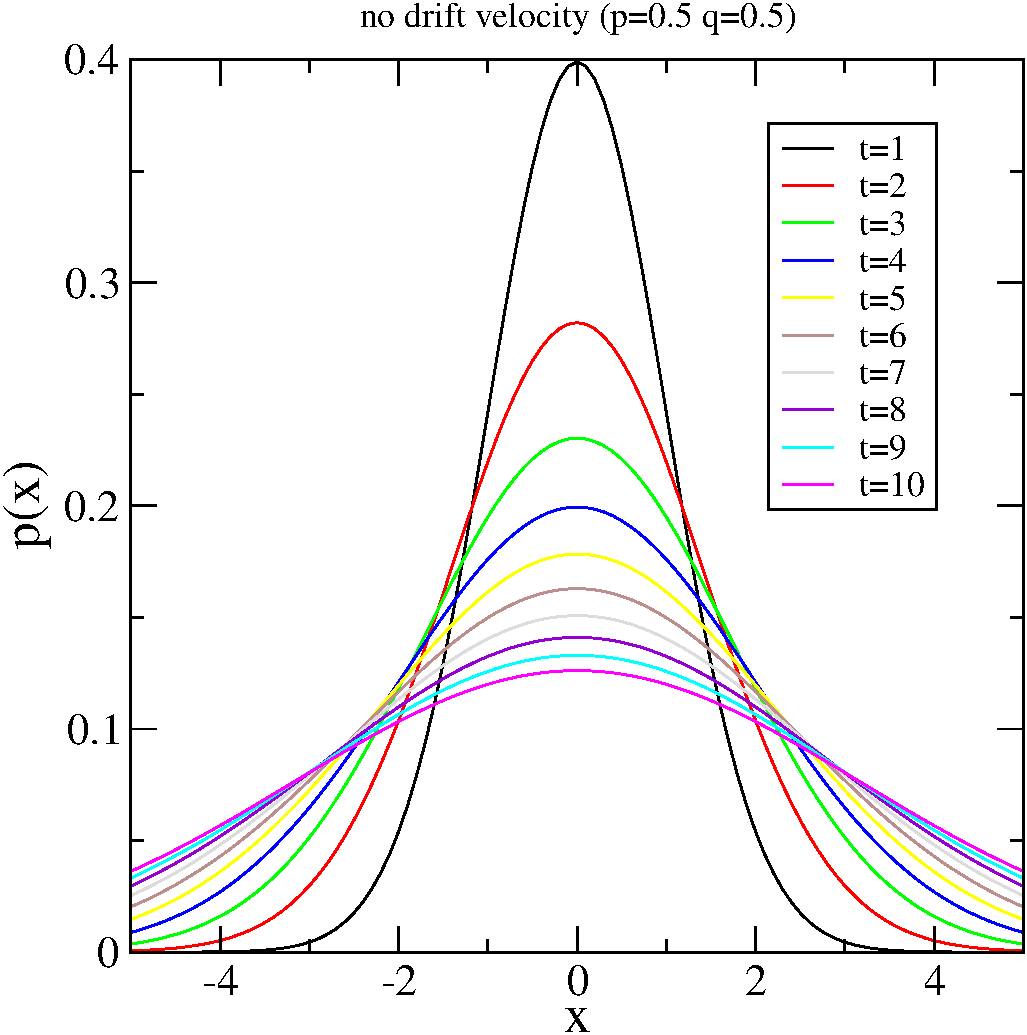
\includegraphics[width=0.45\textwidth]{figs/unit01_diff_zero.pdf}
\end{center}
Here we are considering the special case $p = q = \frac{1}{2}$, for which the drift velocity $\vdr = 0$ and the expectation value is always $\vev{x} = 0$ for any walk time $t$.
However, as time goes on, there is a steady decrease in the probability that the walker will end up at its starting point $x = 0$.
(As in \secref{sec:CLT}, we can extract this probability by integrating the distribution $p(x)$ over the interval $-0.5 \leq x \leq 0.5$.)
Instead, the interval within which we can expect to find the walker (with a constant `one-sigma' or 68\% probability) steadily grows, $-D\sqrt{t} \leq x \leq D\sqrt{t}$, with characteristic dependence on the square root of the time the diffusive process lasts.

Except in the trivial cases $p = 0$ or $q = 0$, diffusion also occurs when the drift velocity is non-zero.
This is shown in the two figures below, considering a low but non-zero drift velocity on the left, and a high drift velocity on the right.
\begin{center} % Don't need centering, but this will provide consistent vertical spacing
  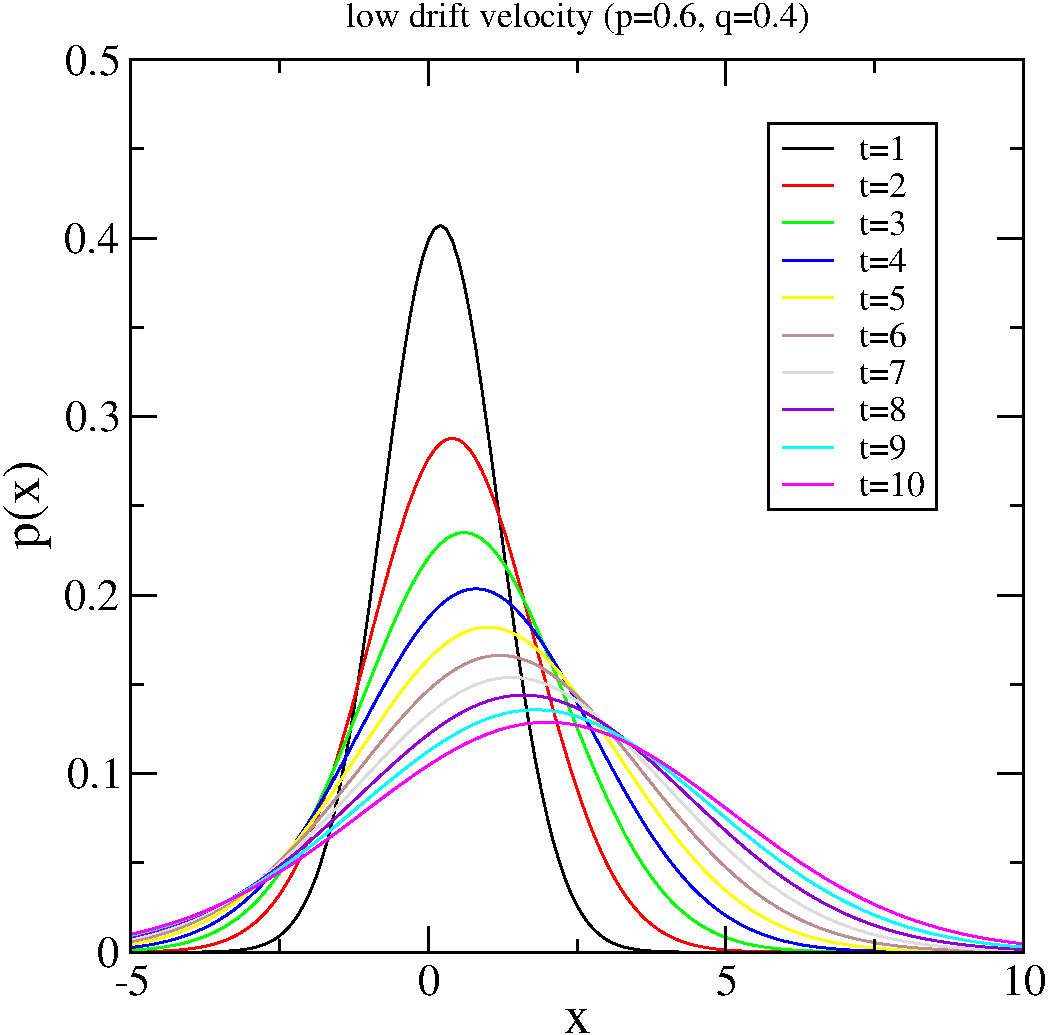
\includegraphics[width=0.45\textwidth]{figs/unit01_diff_low.pdf}\hfill 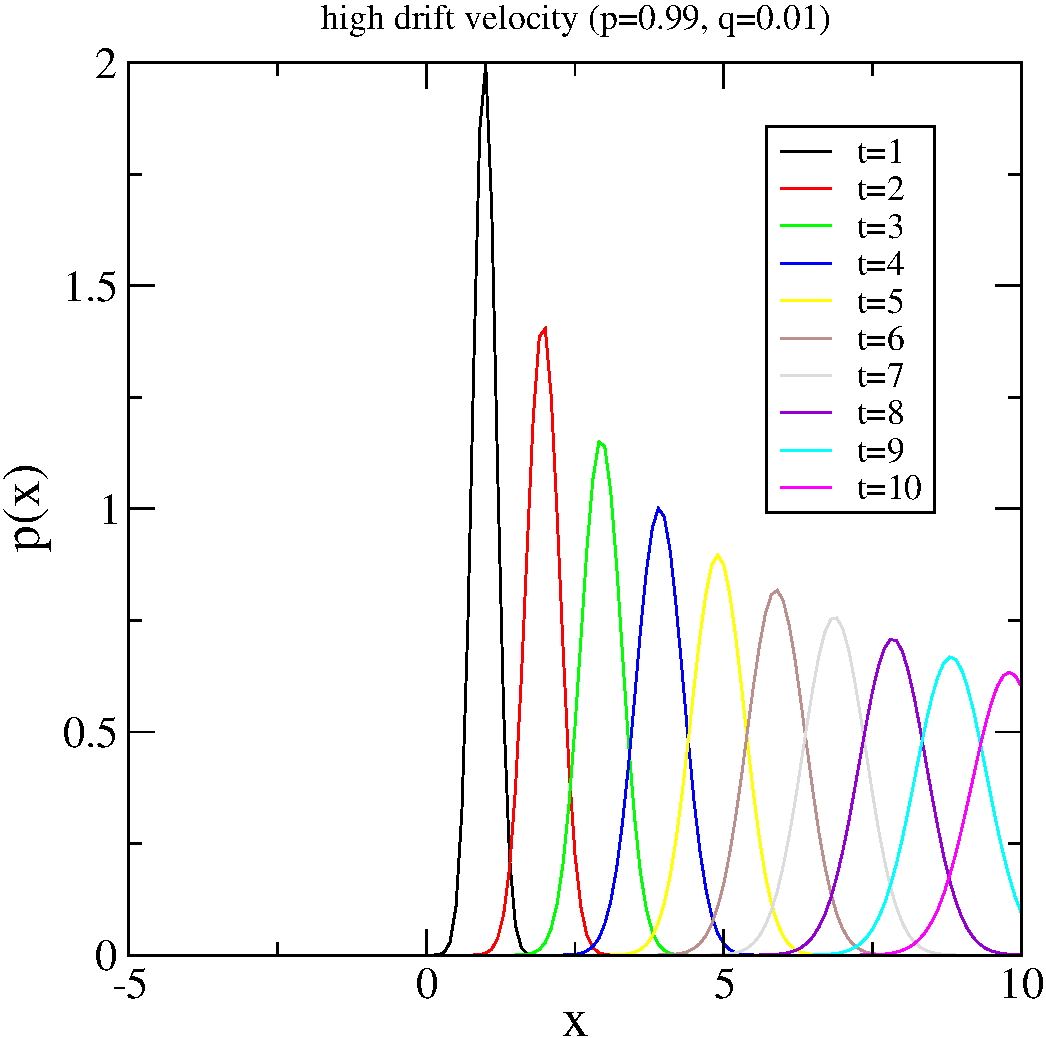
\includegraphics[width=0.45\textwidth]{figs/unit01_diff_high.pdf}
\end{center}
In the figure on the left, each individual probability distribution looks similar to the corresponding one for $\vdr = 0$, but now their central peaks (and expectation values $\vev{x}$) drift steadily to the right.
The distributions in the figure on the right look a bit different, but still diffuse to exhibit shorter and broader peaks as time goes on.

When $p \neq \frac{1}{2}$ so that $\vev{x} \neq 0$, it is interesting to compare the drift in the expectation value against the growth in fluctuations around $\vev{x}$ due to diffusion.
We can do this by considering the following \textit{relative} uncertainty:
\begin{mdframed}
  $\frac{\De x}{\vev{x}} = $ \\[100 pt]
\end{mdframed}
You should find that at large times this ratio vanishes proportionally to $1 / \sqrt{t} \propto 1 / \sqrt{N}$.
Although the absolute uncertainty grows by diffusion, $\De x = D \sqrt{t}$, for $\vdr \neq 0$ the linear drift in the expectation value becomes increasingly dominant as time goes on.
% ------------------------------------------------------------------



% ------------------------------------------------------------------
\subsubsection{\label{sec:RW_CLT}Applying the central limit theorem}
Based on our work in \secref{sec:CLT}, we can see how to apply the central limit theorem to analyze this fixed-step-length random walk in one dimension, for large numbers of steps $N$ or equivalently large times $t = N \De t$.
Each step in the random walk can be considered an independent and identically distributed random variable $x_i$.
The corresponding probability space involves only two possible outcomes: a step of length $\ell = 1$ to the right or to the left with probability $p$ or $q$, respectively.
From this we can easily compute the mean and variance \textit{of the single-step process}:
\begin{mdframed}
  $\mu = \vev{x_i} = $ \\[33 pt]
  $\vev{x_i^2} = $ \\[33 pt]
  $\si^2 = \vev{x_i^2} - \vev{x_i}^2 = $ \\[30 pt]
\end{mdframed}

The final position $x$ of the walker after $N$ steps is exactly the sum over these $x_i$ given in \eq{eq:CLTsum}.
Its probability distribution $p(x)$ from the central limit theorem is therefore obtained directly from these single-step $\mu$ and $\si^2$, which we can also express in terms of the drift velocity and diffusion constant:
\begin{align}
  p(x) & = \frac{1}{\sqrt{2\pi (4Npq)}} \exp\left[-\frac{(x - N(2p - 1))^2}{8Npq}\right] \cr
       & = \frac{1}{\sqrt{2\pi D^2 t}} \exp\left[-\frac{(x - \vdr t)^2}{2D^2 t}\right], \label{eq:RW_CLT}
\end{align}
which was used to produce the three figures above.
We could have jumped straight to the final line by considering \eq{eq:CLT} and noting
\begin{align}
  \label{eq:single_step}
  \vdr t & = N(2p - 1) = N \mu &
  D^2 t & = 4pq \frac{t}{\De t} = N \si^2.
\end{align}
While this dependence on $p$ and $q$ is specific to the particular fixed-step-length random walk we're currently considering, the results $\vdr t = N \mu$ and $D^2 t = N \si^2$ in \eq{eq:single_step} turn out to be generic.
This is remarkable, because it means that the diffusive process as a whole is determined entirely by the single-step mean and variance.
So long as $\mu$ and $\si^2$ are finite, we end up with \eq{eq:RW_CLT} as the large-$t$ probability distribution for any markovian random walk in a single variable $x$.

This result is related to the generality of the law of diffusion (\eq{eq:diff_law}), which we can recognize in the structure of \eq{eq:RW_CLT}.
Since $t > 0$, the exponential in the gaussian distribution $p(x)$ peaks at the drifting expectation value $x = \vdr t = \vev{x}$.
The factor $(x - \vdr t)^2$ simply quantifies the distance from this peak.
As $t$ increases, so does the factor $2D^2 t$ dividing this $(x - \vdr t)^2$, meaning that a larger distance from the peak is needed for the overall argument of the exponential to reach a given value --- in other words, the peak becomes broader.
This in turn requires a shorter peak, reflected in the $\frac{1}{\sqrt{t}}$ in the overall coefficient, which is set by requiring $\int p(x) \; dx = 1$.
In other words, the law of diffusion holds whenever the central limit theorem is applicable.
This requires that the mean and variance of the single-step process are finite, and in the computer project we will numerically investigate the \textit{anomalous diffusion} that occurs when this condition is not satisfied.
% ------------------------------------------------------------------
